%!TEX root = main.tex


Fingerprints are ridge and valley patterns presented on the surface of human fingertips.
%
Fingerprints are used to recognize humans for applications such as verifying an identity claim (i.e., one-to-one search to  unlock a smartphone, for example), or identification (i.e., one-to-many search to find a suspect of a crime, for instance).
%
Typically, to query a fingerprint, the system needs to search and compare the query print with the fingerprints stored in a reference (or enrolled) database.  The size of a reference database can be from thousands to hundreds of millions subjects, depending on the application. For example, the Aaddhar project in India has enrolled 111,98,29,743 persons as of February 18, 2017 \cite{aaddhar}. 
%
As the size of the database grow, the number of comparisons to be made for identification purposes grow, so does the computation time.
%
To mitigate this problem, most fingerprint recognition algorithms first classify a fingerprint into a basic pattern type and then perform fingerprint matching within fingerprints of that type.
%
The major five fingerprint pattern types used today are an extension of the three pattern types (whorl, loop, and Arch) introduced by Henry Faulds (Henry classification system \cite{henry1905classification}) and Sir Francis Galton \cite{galton1892}. in late 19th century. These five pattern types are: arch, left Loop, right Loop, tented arch and whorl, see Fig.\ref{fig.fingerprint_classes}.  
%
Because arch and tented arch only accounts for a small portion(around 6\%) in human, in some automatic fingerprint identification systems, they combine these two classes into one class. 
%
As mentioned above, to manage the computation load, large scale fingerprint identification algorithms employ muti-stage matching whose first step is often filtering based on fingerprint pattern type. As such an accurate fingerprint classification algorithms largely influences the identification accuracy. An error in finger pattern classification will propagate throughout the system, and ultimately result in an recognition error. In this project (paper) we propose an automated fingerprint pattern classification that is not based on feature extraction.

\begin{figure}[!ht]
	\begin{center}
		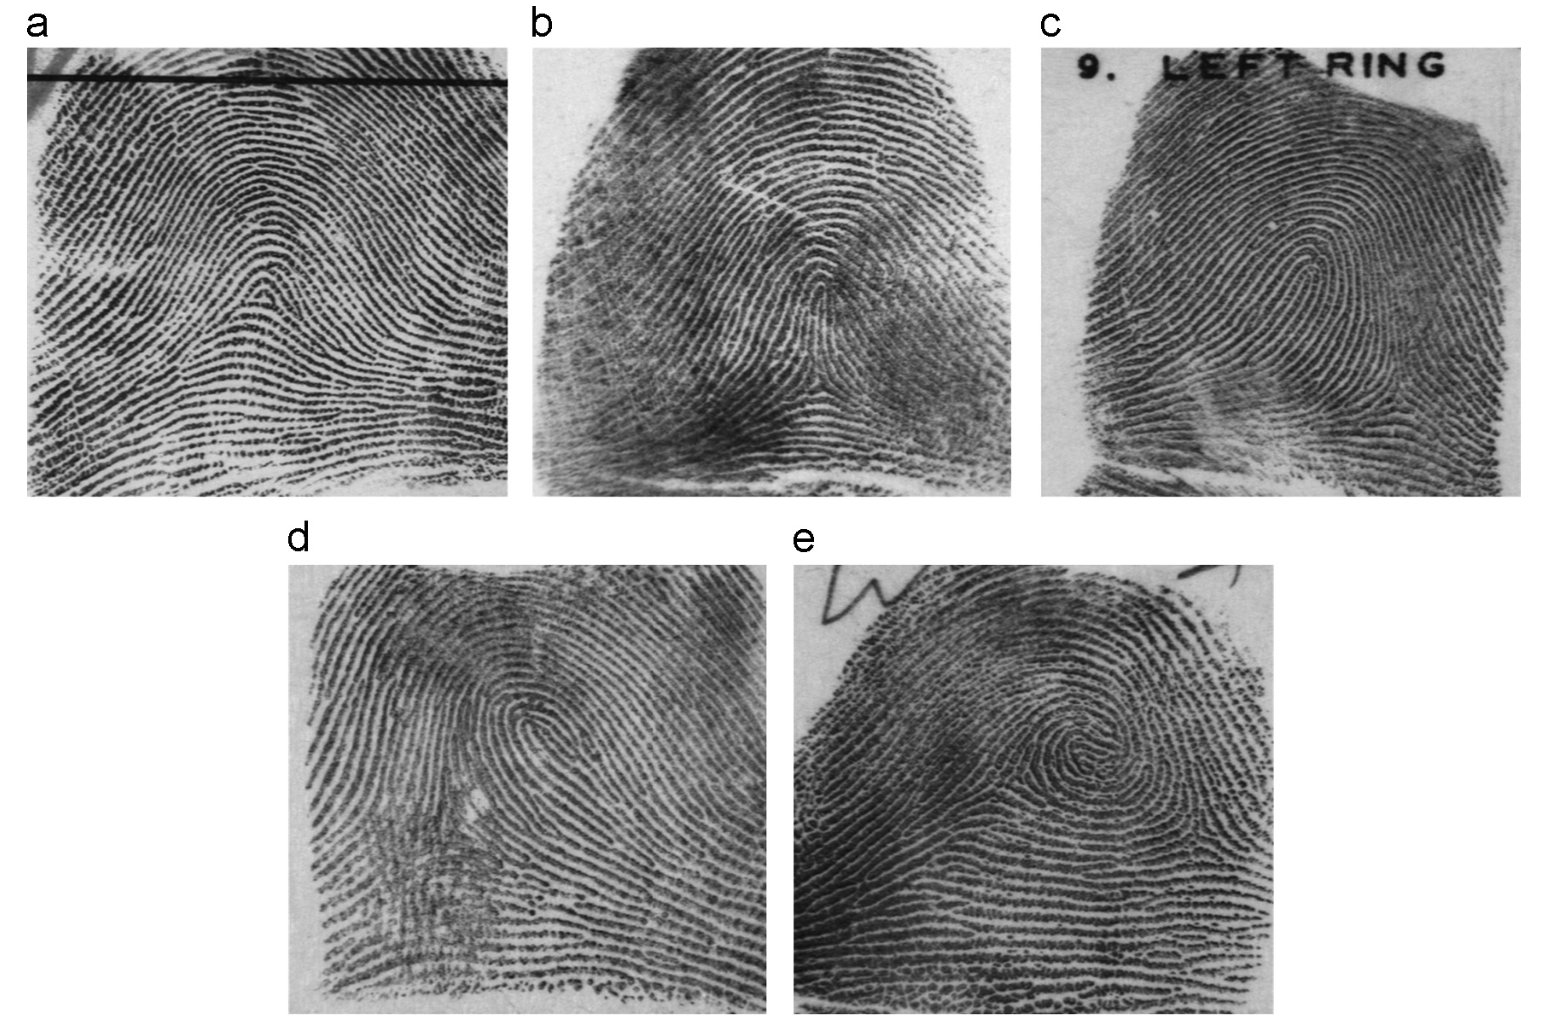
\includegraphics[width=8cm]{fig/Fingerprint_classes.png}
	\end{center}
	\caption{Examples of fingerprint classes: (a) Arch (b) Tented Arch (c) Left Loop (d) Right Loop  (e) Whorl. Note  that tented and tented arch are similar. \cite{cao2013fingerprint}} 
	\label{fig.fingerprint_classes}
\end{figure}

